\documentclass[12pt]{article}
\usepackage{fullpage}
\usepackage{textcomp}
\usepackage{graphicx}
\usepackage{algorithm}
\usepackage{algorithmic}
\usepackage{amsthm}
\newtheorem{lemma}{Lemma}
\usepackage{amsfonts}
\usepackage{amsmath}

\title{Rational Secret Sharing with Conspicuous Secrets}
\author{Craig Gidney}
\date{\today}

\begin{document}

\begin{abstract}
In secret sharing we are asked to split a secret into several shares in such a way that a minimum number of shares is necessary and sufficient to reconstruct the secret. Rational secret sharing considers secret sharing in the context of adversarial players who want to learn the secret but, secondarily, want to prevent other players from learning the secret. 

We present protocols, and bounds on the effectiveness of any protocol, for recombining secret shares in the presence of players who do not want others to learn the secret (rationality), may not want to learn the secret themselves (maliciousness), may be colluding, may have unbounded computational capacity, may be able to synchronize sends (asynchronous/synchronous broadcast), and/or may be able to recognize the secret independently (conspicuousness).

We propose four protocols and analyze their security against players and coalitions who are each rational or malicious. We also prove three results that show protocols using only asynchronous broadcast are less secure than what can be achieved by protocols using synchronous broadcast. 
\end{abstract}

\section{Introduction}

\subsection{Document Map}

- What is secret sharing
- What is conspicuousness
- How does conspicuousness break existing work
- Fuchbauer's protocol
- Characterize rational players
- We present a protocol (ACBP)
- Limits of protocols

\section{Conspicuousness}

A secret is conspicuous if, given a guess at the secret, it is possible to determine if the guess is correct. For example, the combination to a combination lock is inconspicuous when the lock is not present but conspicuous when the lock is present because, given a combination and a lock, you can try the combination on the lock to see if the lock opens.

An inconspicuous secret can be made conspicuous using bit commitment~\cite{Damg02, naor91} (the dealer reveals a commitment to the secret, allowing players to check candidate secrets against the commitment). The opposite transformation, from conspicuousness to inconspicuousness, can't be enforced by a protocol, because players can't be forced to discard information. This asymmetry means conspicuous protocols are more general.

When designing a protocol, the most important consequence of conspicuousness is the inability to rely on a player receiving a candidate secret but only later learning whether or not it is actually the secret. A player can't have the secret but not know that they have the secret. For example, Fuchbauer's et. al.'s blinding protocol~\cite{fuch10} has a per-round shared flag that is set when the previous round's shared secret is the true secret and, as a result, breaks when the secret is conspicuous.

It is possible for conspicuousness to be relative. A secret may be conspicuous to one player but inconspicuous to another. It may be conspicuous to a pair of players but inconspicuous to each individually. It may decrease over time as new information is introduced (e.g. starting a secret sharing protocol forces the secret to be conspicuous to groups of players over the threshold size). When talking about the conspicuousness of a secret this paper always means ``conspicuousness of the secret to each individual player before the protocol starts".

\section{Conspicuousness vs Asynchronous}
\label{Sec:AsympWeak}

Asynchronous secret sharing protocol are less secure in the presence of conspicuous secrets. They must ``sacrifice" at least one player, they are vulnerable to coalitions ``pre-emptively" learning the secret, and rational coalitions may prevent others from learning the secret.

\begin{lemma}\label{Lem:Async:ConspicuousMustSacrifice}If the secret is conspicuous, all players are rational, and communication is asynchronous, then at least one player will not learn the secret.\end{lemma}
\begin{proof}
We will prove this result by contradiction. Assume all players learn the secret.

The protocol is divided into rounds with a single sender per round, by definition from subsection~\ref{Def:Broadcast}. Let $r$ be the first round such that, at the end of round $r$, all players will eventually know the secret even if the others stop cooperating. Let $s$ be the sender of round $r$'s message.

$s$ must be able to compute the secret before round $r$, because $s$ must be able to compute the secret after round $r$ (we assumed all players could) but will receive no new information (due to being the single sender).

$s$ will not send a correct message in round $r$. $s$ can compute the secret before round $r$ and $s$ knows this fact, because the secret is conspicuous. But, knowing this fact, $s$ has no incentive to send a correct message during round $r$. Doing so could only help the other players learn the secret which, because $s$ is rational, $s$ wants to prevent from happening.

There is no round where all players will eventually know the secret. The definition of $r$ is contradicated by $s$ not sending a correct message in round $r$. $r$ was defined to be the first round where all players were guaranteed to eventually know the secret even if the others stopped cooperating, but now the previous round also satisfies that constraint (unless $r=0$, in which case the protocol is not correct because players can learn the secret independently).

At least one player will not learn the secret. Otherwise there would be a round where all players would eventually know the secret.
\end{proof}

\begin{lemma}\label{Lem:Async:CoalitionsMayPreempt}If the secret is conspicuous, all players are rational, and communication is asynchronous, then, given the total number of players, there is a probability bounded away from 0 that a coalition of randomly chosen players will learn the secret before any individual player could have.\end{lemma}
\begin{proof}
An asynchronous protocol is divided into rounds with a single sender per round, by definition from subsection~\ref{Def:Broadcast}. 
Let $n$ be the number of players.
Let $C$ be a rational coalition of players, selected randomly, with size less than the threshold $t$.
Let $r$ be the first round where a player would have learned the secret if there were no collusion.
Let $L$ be the set of learners: players who learn the secret in round $r$.
Let $s$ be the sender of round $r$'s message.
The sender cannot be one of the learners because the sender is receiving no new information during round $r$.

If the sender and at least one of the learners are in the coalition, then the coalition can internally simulate sending round $r$'s message before round $r$ occurs and thereby pre-emptively learn the secret before any individual player could. The probability of this occurring is $\frac{|C|}{n} \times \left(1 - \frac{\binom{n - |C|}{|L|}}{\binom{n - 1}{|L|}}\right)$. This function varies with the size of $L$, which depends on the protocol. Higher values of $L$ give higher probabilities, so a lower bound for any protocol can be computed by setting $|L|$ to its minimum value: $1$. This gives a probability of $\frac{|C| \times (|C| - 1)}{n \times (n-1)}$, which is bounded away from $0$ when $n$ is fixed.
\end{proof}

\begin{lemma}\label{Lem:Async:NoConspGoodRatImmune}If the secret is conspicuous, all players are rational, and communication is asynchronous, then either at most $\lceil \frac{n}{2} \rceil$ of the players learn the secret or a rational coalition may reduce the number of players that learn the secret.\end{lemma}
\begin{proof}
The protocol is divided into rounds with a single sender per round, by definition from subsection~\ref{Def:Broadcast}. Before a round $r$ a player $p$ has some minimum number $m(p, r)$ of other players that must continue cooperating in order for $p$ to learn the secret. If $p$ learns the secret when round $r$ finishes, then $m(p, r) = 1$, because $p$ must have received a message from the round's sender that allowed $p$ to learn the secret, and $m(p, r+1) = 0$. The number of cooperating players a given player needs can decrease by either 1 or 0 each round (for example, a message may be either a definitive share or a check message), so we can further derive that $m(p, r-i) \leq 1+i$.

Let $h(r)$ be the minimum value of $m(p, r)$ for any player on round $r$. If at least one player learns the secret, and the protocol satisfies the basic correctness requirement that $t$ players are needed in order for any to learn the secret, then for any $i \in [0, t]$ there will be a round where $h(r) = i$.

Suppose a rational coalition $C$ has size $|C|$ satisfying $1 < |C| < t$. Let $r_0$ be the smallest round such that $h(r) = |C|-1$. In round $r_0$ there is a player who depends on at most $|C|-1$ other players. If that player is in the coalition, and the potential dependees are the other players in the coalition, then the coalition can learn the secret and defect. This leaves at most $n-|C|$ cooperating players, all of whom need at least $|C|-1$ other players to be present in order to learn the secret due to how we choose $r_0$. If $n < 2 |C|$, then they can't learn the secret and will fail.

When the number of players who would have learned the secret if the protocol had been run without the coalition is larger than $\lceil \frac{n}{2} \rceil$, they can't all be placed in the coalition. Either at most $\lceil \frac{n}{2} \rceil$ players learn the secret or the coalition defecting on round $r$ causes fewer players to learn the secret than if the coalition had not been present.
\end{proof}

\section{Existing Protocols are Vulnerable to Conspicuous Secrets}

\section{Asynchronous Conspicuous Blinding Protocol}
\label{Sec:ACBP}

The protocol presented in this subsection, named ACBP (asynchronous conspicuous blinding protocol), is an asynchronous protocol for conspicuous secrets. It guarantees that at most $t-1$ non-colluding rational players are sacrificed, but allows for only $1$ player to be sacrificed if all players are non-colluding and rational.

\subsection{Overview}

ACBP is similar to the protocol by Fuchbauer et. al \cite{fuch10}, except the definitive round is ``spread out'', meaning different players learn the secret after different rounds. This allows players who send later to be incentivized into participating for one more round by delaying when they learn the secret.
 
ACBP is based on a sequence of check rounds followed by a block of $n$ definitive rounds during which a player learns shares of the true secret. Players take turns sending messages in a round robin format. The start of the block of definitive rounds is different for each player and chosen so that, when they are supposed to send their last message, they will need a specified number of additional shares before they learn the secret. Each round every player sends a message created by a verifiable random function (VRF). Each player takes received messages and offsets them to create round shares. The offset applied is different for each ordered pair of sender and receiver, but does not depend on the round. Both the offsets and VRFs are chosen beforehand by a dealer.

Before a player's definitive block of rounds the round shares they compute are random. The offsets and VRFs are chosen by the dealer to ensure that during the player's definitive block of rounds the round shares they compute are the Y coordinates of Shamir shares for the secret with a threshold of $t$. Players recognize the definitive round by combining the round shares and matching the result against a bit commitment to the secret provided by the dealer. Each player's definitive block of rounds is positioned so that the earliest round they can learn the secret is a specified number $\delta$, called the ``share shortage", of rounds after a round where they send a message.

See Algorithms \ref{alg:ACBP:Dealer} and \ref{alg:ACBP:Player} and Figure \ref{img:ex:ACBP} for details.

\begin{algorithm}
  \caption{Dealer Protocol for ACBP}
  \label{alg:ACBP:Dealer}
  \begin{algorithmic}
    \INPUT Finite field $\mathbb{F}$, number of shares $n$, and threshold $t$
    \INPUT Share shortage $\delta$ satisfying $0 < \delta < t$
    \INPUT Marginal probability of termination $\alpha$
    \INPUT Verifiable random function scheme $VRFS$ and commitment scheme $CS$
    \INPUT Secret value $s$ from the finite field $\mathbb{F}$
    \OUTPUT An ordered list of $n$ ACBP shares for the secret $s$ with a threshold of $t$
    \STATE Create a commitment $c$ to the secret $s$
    	$$c = CS.CreateCommitment(s)$$
    \STATE Create ordered lists $V$ and $G$ of $n$ public ($V$) and private ($G$) VRFS key pairs
    	$$V_i, G_i = VRFS.NewKeyPair()$$
    \STATE Pick the earliest definitive round of any share $b$ 
	    $$b = Random(UniformDistribution([0,n))) + Random(Geometric(\alpha))$$
    \STATE Compute the starting round $r_i$ satisfying $r_i \geq b$ of each share's block of definitive rounds based on the desired share shortage by also satisfying $r_i + t - 1 - \delta = i \pmod{n}$
  	    $$r_i = b + ((i-b-t+\delta+1) \text{ } mod \text{ } n)$$
    \STATE Create $n$ ordered lists $S_i$ of $n$ Shamir shares (points) $S_{i,j}$ with threshold $t$ for the secret
  	    $$S_i = CreateShamirShares(s, \mathbb{F}, n, t) \text{ } for \text{ } i \in [1, n]$$
  	    $$XOfPoint(S_{i,j}) = j \text{ } for \text{ } i,j \in [1, n]$$
    \STATE Compute the $n$ ordered lists $Y_i$ of $n$ offsets $Y_{i,j}$
  	    $$Y_{i,j} = VRFS.ValueOf(G_j, r_i + (j-r_i \pmod{n})) + S_{i,j}$$
    \STATE Return the list $R$ of $n$ ACBP shares composed of the commitment, all public keys, share-specific offsets, an index, and a private key
    	$$R_i = (c, V, Y_i, i, G_i)$$
  \end{algorithmic}
\end{algorithm}
\begin{algorithm}
  \caption{Player Protocol for ACBP}
  \label{alg:ACBP:Player}
  \begin{algorithmic}
    \INPUT Finite field $\mathbb{F}$
    \INPUT Total number of shares $n$ and threshold $t$
    \INPUT Verifiable random function scheme $VRFS$ and commitment scheme $CS$
    \INPUT Share index $i \in [1, n]$
    \INPUT VRFS private key $G_i$
    \INPUT Ordered list $V$ of $n$ VRFS public keys
    \INPUT Ordered list $Y_i$ of $n$ offsets
    \INPUT Secret commitment $c$
    \OUTPUT Secret value or failure
    \STATE Mark all players, identified by indexes in $[1,n]$, including ourselves, as cooperating
    \STATE Let $Q$ be an empty queue of points in $\mathbb{F}^2$
    \STATE Let $r = 1$
    \WHILE {true}
	  \STATE If fewer than $t$ players are marked as cooperating then exit with failure
	  \STATE Let $x$ be the player with index $j$ satisfying $j \equiv r \pmod{n}$
	  \IF {$j = i$} 
	  	 \STATE Broadcast the message $VRFS.ValueAndProof(G_i, r)$ to all cooperating players
	  \ENDIF
	  \STATE Let $m, w$ be the message value and proof received from $x$ (if any) in round $r$
	  \STATE If $x$ sent no message or a message failing $VRFS.Verify(V_j, m, w)$ then mark $x$ as non-cooperating
	  \STATE If $x$ is marked as non-cooperating then skip to the next round
	  \STATE Enqueue the point $(j, m + Y_{i,j})$ into $Q$
      \STATE If $Q$ has more than $t$ items then dequeue the oldest item from $Q$
	  \IF {$Q$ has $t$ items}
	   	\STATE Let $P$ be the polynomial interpolated from the points in $Q$
	    \STATE If $CS.Matches(c, P(0))$ then exit with the secret $P(0)$
	  \ENDIF
      \STATE Increment $r$ by $1$
	\ENDWHILE
  \end{algorithmic}
\end{algorithm}
\begin{figure}
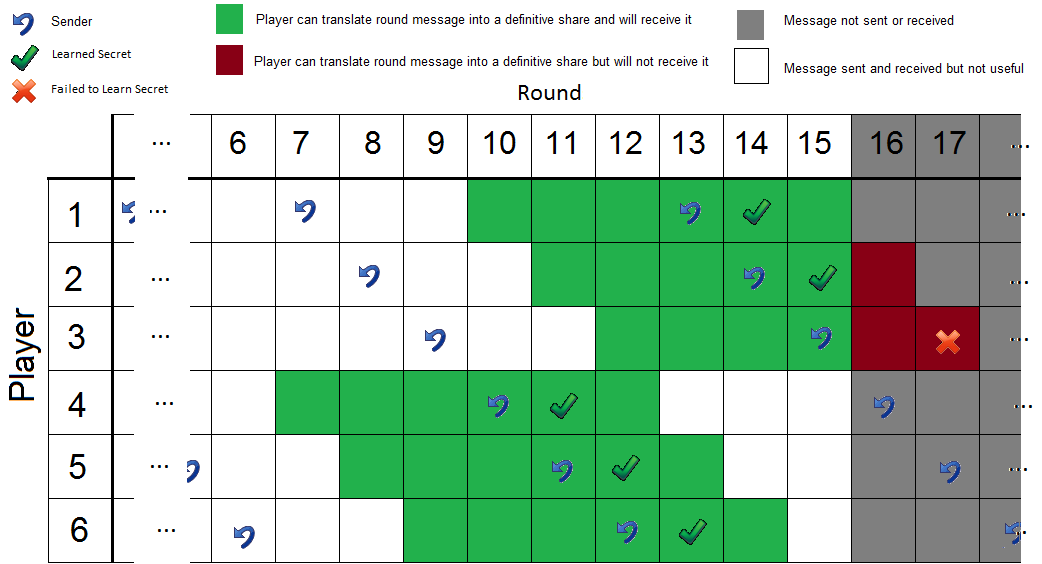
\includegraphics[width=\textwidth]{../../Graphics/AsyncVerifiedSecret_n6t5d1.png}
\caption[Shares learned by players running ACBP]{Representation of shares learned by players running ACBP with $n=6, t=5, \delta=1$. One player does not receive enough definitive shares and is sacrificed.}
\label{img:ex:ACBP}
\end{figure}

\subsection{Analysis}

ACBP is less efficient than Fuchbauer et al's protocol. If the number of players is $n$, the threshold is $t$, the marginal first definitive round probability is $\alpha$, the share shortage is $\delta$, and the costs of the commitment scheme, verifiable random function scheme, and Shamir's share scheme are represented as $CS$, $VRFS$ and $Shamir(t, n)$, then the asymptotic expected time is $O(VRFS  \times n^2 + CS + Shamir(t, n) \times n)$ for the dealer and $O((n + \frac{1}{\alpha}) \times (CS + VRFS + Shamir(t, t)))$ for the players. The practical costs depend primarily on the efficiency of the implementations of the VRF and Shamir schemes. ACBP's shares each contain $O(n)$ information.

ACBP is immune to malicious coalitions, as shown in Lemma~\ref{Lem:ACBP:MalImmune}, because a malicious player can do no more harm than an abstaining player. However, we must emphasize that this result is somewhat misleading because ACBP has the related undesirable property that \emph{abstaining players can do some harm}. Lemma~\ref{Lem:ACBP:AbstainBad} shows it is possible for one abstaining player to cause one other player to not learn the secret. ACBP is immune to malicious coalitions, despite the fact that changing a rational player to a malicious player may cause another player not to learn the secret, because changing the same rational player to an absent player has the same effect.

ACBP is not immune to rational coalitions. This is a consequence of Lemma~\ref{Lem:Async:NoConspGoodRatImmune} and the fact that ACBP allows more than $\lceil \frac{n}{2} \rceil$ players to learn the secret. In particular, rational coalitions with size greater than $\delta$ may have enough ``future" shares to defect before they reveal any definitive shares to other players. The share shortage $\delta$'s value is a trade-off between stronger resilience against rational coalitions and sacrificing fewer players. Coalitions tend to decrease the number of players who learn the secret, although it is also possible for a coalition to \emph{increase} the number of players who learn the secret by saving a colluder from being sacrificed.

One interesting property of ACBP is that non-colluding players experience no temptation to defect, as shown in Lemma~\ref{Lem:ACBP:SoloTemptNone}. This is possible because some players are sacrificed. Instead of guaranteeing all cooperators learn the secret, ACBP guarantees all defectors do not learn the secret. A non-colluding rational player's optimal strategy is to cooperate, even if $\alpha$ is almost 1.

If at least $t$ players are present and want to learn the secret, running ACBP ensures at least $1$ of them learns it. This is a consequence of ACBP's immunity to malicious coalitions and Lemma~\ref{Lem:ACBP:SomeDeltaLose}, which shows that if there are at least $t$ cooperating rational players, then at most $t-1$ of them are sacrificed. Lemma~\ref{Lem:ACBP:AllDeltaLose} shows that if all players are cooperating and rational, then exactly $\delta$ of them are sacrificed.

\begin{lemma}\label{Lem:ABPC:MarginalAtMostAlpha}The marginal probability of a given next round being the definitive round is at most $\alpha$.\end{lemma}
See Appendix \ref{Appendix:ACBP:Probabilities:MarginalFirstDefinitiveRoundBelowAlpha}, which shows that the probability distribution of the sum of a random value from a uniform distribution over $[1,n]$ and a geometric distribution parameterized by $\alpha$ never exceeds $\alpha$.

\begin{lemma}\label{Lem:ACBP:FairSacrificeBefore}Before the player protocol runs, the probability of a player being sacrificed is independent of their share index.\end{lemma}
\begin{proof}
Whether or not the player given index $i$ by the dealer is sacrificed depends on their index $i$, the first definitive round $b$, and the share shortage $\delta$. At the end of round $b+t-1$ the player with index satisfying $i = b+t-1-\delta \pmod{n}$ will learn the secret. For the following $n-\delta-1$ rounds the player who learns the secret has the next index, cycling from $1$ to $n$. The remaining $\delta$ players will not learn the secret and are sacrificed. If the value of $b$ is increased by $1$, the sacrificed indexes also increase by $1 \pmod{n}$. If the value of $b$ increases by $n$, the sacrificed indexes are unaffected. The distribution of the offset of the block of sacrificed indexes is uniform if the distribution of $b \pmod{n}$ is uniform.

The probability of the first definitive round $b$ being at least $r$ and in a given equivalence class of integers mod $n$ is $F^{*}(r) = \frac{1}{n} \times (1-\alpha)^{0 \uparrow (r - n + 1)}$ (see Appendix \ref{Appendix:ACBP:Probabilities:MarginalFirstDefinitiveRoundBelowAlpha}). When $r < n$ this simplifies to $\frac{1}{n}$, meaning the first definitive round has an equal probability of landing in each equivalence class. Therefore the offset of the block of sacrificed indexes is also uniformly distributed and the probability of a given player being sacrificed is also uniformly $\frac{1}{n}$, independent of their share index.
\end{proof}

\begin{lemma}\label{Lem:ACBP:FairerDuringWithSmallAlpha}By choosing a small enough $\alpha$, the conditional probability of a round's sender being sacrificed, given that the current round has been reached, can be made arbitrarily close to uniform.\end{lemma}
See Appendix \ref{Appendix:ACBP:Probabilities:MarginalEquivalenceClassDefinitiveRoundApproaches1OverN}, which shows that the probability distribution of the equivalence classes of the first definitive round modulo $n$ limits to $\frac{1}{n}$ as $\alpha$ approaches $0$ from the positive direction.

\begin{lemma}\label{Lem:ACBP:SoloTemptNone}Non-colluding rational players who defect do not learn the secret.\end{lemma}
\begin{proof}
When a player sends for the final time, the dealer has positioned their block of definitive rounds such that they will need at least $\delta$ more shares before they can learn the secret. If they defect instead of sending, other players will stop sending them messages. Since they are not colluding and not being sent messages from which they can derive shares, they won't be able to access the definitive shares they need. Therefore if they defect they will not learn the secret.
\end{proof}

\begin{lemma}\label{Lem:ACBP:AllDeltaLose}If all players are non-colluding and cooperating until they learn the secret, then exactly $n-\delta$ players will learn the secret.\end{lemma}
\begin{proof}
When all players cooperate there will be exactly one player who will receive $i$ definitive shares, counting their own, for each $i$ in $[t-\delta, n-1]$. The remaining $t-\delta$ players will receive $n$ definitive shares. This occurs as a consequence of players defecting as they learn the secret and the positioning of the definitive shares by the dealer (see Figure \ref{img:ex:ACBP} for a visual example).

Non-colluding players learn the secret if and only if they receive $t$ or more definitive shares. The range $[t-\delta, n-1]$ contains $n-1-t+1$ values greater than or equal to $t$ and $n \geq t$ so in total there are $(n-1-t+1) + (t-\delta) = n-\delta$ players who will receive enough definitive shares to learn the secret.
\end{proof}

\begin{lemma}Cooperating is a Nash equilibrium for non-colluding rational players.\end{lemma}
\begin{proof}
When it is a player's turn to send they can send the right message, send a fake message, or send no message. Defecting is sending a fake message or no message. If a player sends no message, then their defection is always detected. If they send an incorrect message, then their defection is detected with an arbitrarily high probability determined by the VRF scheme.

A non-colluding rational player will not learn the secret if they defect, by Lemma~\ref{Lem:ACBP:SoloTemptNone}. If they cooperate they will learn the secret with non-zero probability, since the other players are assumed to be following the equilibrium strategy of cooperating, and only some players are sacrificed (if $\alpha$ is small and all other players are cooperating and non-colluding, then, by Lemmas~\ref{Lem:ACBP:FairerDuringWithSmallAlpha} and \ref{Lem:ACBP:AllDeltaLose}, the probability is approximately $\frac{\delta}{n}$). The payoff of cooperating is larger than the payoff of defecting, so non-colluding rational players will follow the equilibrium strategy of cooperating.

Therefore, because a rational player's best strategy is to cooperate when all other rational players cooperate, cooperating is a Nash equilibrium for non-colluding rational players. 
\end{proof}

\begin{lemma}\label{Lem:ACBP:SomeDeltaLose}If ACBP is run with $x \in [t,n]$ non-colluding rational players, then the number of those players who learn the secret is in $(x-t, x-\delta]$.\end{lemma}
\begin{proof}
When a player is absent or defects before the definitive rounds, they decrease the number of definitive shares that will be received by players who depended upon the defector/absentee by 1. Conversely, if a player is present and sends the right message until they learn the secret they will increase the number of definitive shares that will be received by players who depended upon them by 1. Adding players can only increase the number of players who will learn the secret. Thus we can prove a lower bound on the number of players who learn the secret without considering cases where additional players, on top of the non-colluding rational players, are present.

First we will show the lower bound. Suppose the protocol is run with $x \in [t,n]$ players. For every pair of present players $p_1, p_2$, where $p_1$ would have learned the secret before $p_2$ if all players were present, $p_2$ will give a definitive share to $p_1$. It is possible for $p_1$ to also give a definitive share to $p_2$, but not necessary. This is a consequence of the players learning the secret in the same cyclic order as sending messages. There is a distinct player who will learn at least $j$ definitive shares for each value of $j \in [1, i]$. For example, the player who would have learned the secret first out of the present players, if all absent and present players had been present and cooperating, will receive at least $x$ shares including their own. There are $x-t+1$ values greater than or equal to $t$ in $[1,x]$, so more than $x-t$ players will learn at least $t$ definitive shares, and learn the secret.

The upper bound is a consequence of the fact that a player needs $\delta$ shares when they send their final message. The final $\delta$ senders need more shares than the number of remaining messages, so they don't learn the secret. At most $x-\delta$ players will learn the secret.  
\end{proof}

\begin{lemma}\label{Lem:ACBP:AbstainBad}An abstaining player may decrease the number of players who learn the secret by 2.\end{lemma}
\begin{proof}
When a player abstains from participating in the protocol, they decrease the number of definitive shares that will be received by each player who depended upon the abstainer by one. If the abstaining player would have learned the secret and the dependent players includes a player who was only receiving $t$ definitive shares, then two fewer players will learn the secret.

Consider the case where all players are present, rational, non-colluding, and at least two learn the secret. If the before-last player who would have learned the secret abstains, then the last player who would have learned the secret will receive one fewer definitive shares. But the last player to learn the secret would only have had $t$ definitive shares, and so they will not learn the secret if the before-last player abstained.

When the before last player who would have learned the secret abstains, both the last and before-last players who would have learned the secret fail to learn the secret. Therefore a player may decrease the number of players (including themselves) who learn the secret by two by choosing to abstain.
\end{proof}

\begin{lemma}\label{Lem:ACBP:MalImmune}ACBP is immune to malicious coalitions.\end{lemma}
\begin{proof}
The VRF scheme ensures that, when a malicious player does not cooperate, they are detected with arbitrarily high probability. When a defector is detected, the player algorithm ignores them by not sending them messages and discarding any messages they send. Therefore malicious coalitions either cooperate or, with arbitrarily high probability, are ignored and have an effect equivalent to absent players. That is the definition of malicious immunity from subsection~\ref{Def:Immunity}.
\end{proof}

\subsubsection{Summary}

ACBP generalizes SBP to use only asynchronous broadcast. Its notable improvement over existing asynchronous protocols is allowing for the secret to be conspicuous without ensuring the sacrifice of $t-1$ players even when none are colluding. ACBP may sacrifice as many as $t-1$ non-colluding players but can also sacrifice as few as $1$ (the minimum set by Lemma~\ref{Lem:Async:ConspicuousMustSacrifice}).

ACBP is immune to malicious coalitions, in that their effect on the outcome is equivalent to abstaining players, but may sacrifice an additional player when a player chooses to abstain. ACBP is a conspicuous asynchronous protocol and allows for more than a strict majority of players to learn the secret which, by Lemma~\ref{Lem:Async:NoConspGoodRatImmune}, means it is not immune to rational coalitions.

There appears to be significant room for improvement over ACBP. For example, we are considering using Maleka S's TRSS~\cite{MalekaS_08} protocol with ACBP as the second stage. This guarantees that, if there is $1$ non-colluding rational player, at most $1$ non-colluding player is sacrificed and all other players can learn the secret. However, TRSS with ACBP is ``less fair" because it favors colluding much more heavily than ACBP. In particular, if there is a single non-colluding player, then TRSS with ACBP is guaranteed to sacrifice that player.






\section{Conclusion}
\label{section:Conclusion}

Four protocols were presented by this thesis: a synchronous protocol for bounded opponents (SBP), a synchronous protocol for unbounded opponents and inconspicuous secrets (SUIP), an asynchronous protocol for bounded opponents and conspicuous secrets (ACBP), and an asynchronous protocol for bounded opponents and inconspicuous secrets (ABIP). Each of these protocols has notable improvements over existing work. SBP is immune to malicious coalitions. SUIP is more secure than existing list-based protocols due to making the short case exceptional instead of required, its security relies only on missing information (not computational difficulty) and it is immune to malicious coalitions. ACBP can sacrifice fewer than $t-1$ players when the secret is conspicuous and is immune to malicious coalitions. ABIP is immune to malicious coalitions up to size $n-t$.

This thesis also proved three limitations of asynchronous protocols. There is always a chance that a coalition may learn the secret earlier than any non-colluding player could have. If the secret is conspicuous and no players are colluding, then at least one player will be ``sacrificed" and not learn the secret. If the secret is conspicuous and the protocol allows for more than $\lceil \frac{n}{2} \rceil$ players to learn the secret, then the protocol is not immune to rational coalitions.





\bibliographystyle{plain}
\bibliography{../../References/_refs}


\appendix
\section{Calculating Probability Distributions related to ACBP }
\label{Appendix:ACBP:Probabilities}

The notation $a \uparrow b$ means $max(a, b)$. The $\uparrow$ operator has precedence between addition and multiplication. For example, $1 + 2 \uparrow 3 \times 4 = 1 + max(2, 3 \times 4) = 13$.

\subsection{Probability Distribution of First Definitive Round}
\label{Appendix:ACBP:Probabilities:FirstDefinitiveRound}

The first definitive round of ACBP is generated by adding a geometric distribution parameterized by $\alpha$ to a uniform distribution over $(0, n]$. Its probability distribution is represented here by the function $F$ and can be simplified as follows:

\begin{align*}
F(r)
  &= \sum_{i=0 \uparrow (r-n+1)}^r \frac{1}{n} \times \alpha \times (1-\alpha)^i
\\&= \frac{\alpha}{n} \times \frac{(1-\alpha)^{0 \uparrow (r-n+1)} - (1-\alpha)^{r+1}}{1 - (1-\alpha)}
\\&= \frac{1}{n} \times ((1-\alpha)^{0 \uparrow (r-n+1)} - (1-\alpha)^{r+1})
\end{align*}

\subsection{Marginal Probability Distribution of First Definitive Round Never Exceeds $\alpha$}
\label{Appendix:ACBP:Probabilities:MarginalFirstDefinitiveRoundBelowAlpha}

During ACBP players believe that the definitive round will be the next round with some probability. The marginal probability of the definitive round being the next round, given that all previous rounds were not the definitive round, is represented here by the function $F'$. We simplify $F'$ in order to show that it is never larger than $\alpha$.

\begin{align*}
F'(r)
  &= \frac{F(r)}{\sum_{i=r}^{\infty} F(i)}
\\&= \frac{(1-\alpha)^{0 \uparrow (r-n+1)} - (1-\alpha)^{r+1}}{\sum_{i=r}^{\infty} ((1-\alpha)^{0 \uparrow (i-n+1)} - (1-\alpha)^{i+1})}
\\&= \frac{(1-\alpha)^{0 \uparrow (r-n+1)} - (1-\alpha)^{r+1}}{(\sum_{i=r-n+1}^{-1} (1-\alpha)^0) + (\sum_{i=r \uparrow (r-n+1)}^{\infty} (1-\alpha)^i) - (\sum_{i=0}^{\infty} (1-\alpha)^{i+1})}
\\&= \frac{(1-\alpha)^{0 \uparrow (r-n+1)} - (1-\alpha)^{r+1}}{(0 \uparrow (-1 - (r-n+1) + 1)) + (\frac{(1-\alpha)^{0 \uparrow (r-n+1)}}{1 - (1-\alpha)}) - (\frac{(1-\alpha)^{r+1}}{1 - (1-\alpha)})}
\\&= \alpha \times \frac{(1-\alpha)^{0 \uparrow (r-n+1)} - (1-\alpha)^{r+1}}{\alpha \times (0 \uparrow -(r-n+1)) + (1-\alpha)^{0 \uparrow (r-n+1)} - (1-\alpha)^{r+1}}
\end{align*}

Case 1: $r-n+1 \geq 0$
\begin{align*}
F'(r)
  &= \alpha \times \frac{(1-\alpha)^{r-n+1} - (1-\alpha)^{r+1}}{\alpha \times 0 + (1-\alpha)^{r-n+1} - (1-\alpha)^{r+1}}
\\&= \alpha \times \frac{(1-\alpha)^{-n} - (1-\alpha)^{0}}{(1-\alpha)^{-n} - (1-\alpha)^{0}}
\\&= \alpha
\\&\leq \alpha
\end{align*}

Case 2: $r-n+1 \leq 0$
\begin{align*}
F'(r)
  &= \alpha \times \frac{(1-\alpha)^0 - (1-\alpha)^{r+1}}{\alpha \times -(r-n+1) + (1-\alpha)^0 - (1-\alpha)^{r+1}}
\\&= \alpha \times \frac{1 - (1-\alpha)^{r+1}}{\alpha \times -(r-n+1) + 1 - (1-\alpha)^{r+1}}
\\&= \alpha \times (1 + \frac{-\alpha \times -(r-n+1)}{\alpha \times -(r-n+1) + 1 - (1-\alpha)^{r+1}})
\\&\leq \alpha
\end{align*}

\subsection{Marginal Probability of Equivalence Classes of First Definitive Round Limits to $\frac{1}{n}$ as $\alpha$ Approaches $0$}
\label{Appendix:ACBP:Probabilities:MarginalEquivalenceClassDefinitiveRoundApproaches1OverN}

The value of the first definitive round, modulo $n$, is important for determining which players are sacrificed. The probability of the first definitive round being in the same equivalence class, and at least as large, as a given round $r$ is represented here by $F^{*}$. We simplify $F^{*}$ for future use. 

\begin{align*}
F^{*}(r)
  &= \sum_{i=0}^{\infty} F(r + i \times n)
\\&= \frac{1}{n} \times \sum_{i=0}^{\infty} ((1-\alpha)^{0 \uparrow (r + i \times n - n + 1)} - (1-\alpha)^{r + i \times n + 1})
\\&= \frac{1}{n} \times (((1-\alpha)^{0 \uparrow (r + 0 \times n - n + 1)}) + (\sum_{i=1}^{\infty} (1-\alpha)^{0 \uparrow (r + i \times n - n + 1)}) - (\sum_{i=0}^{\infty} (1-\alpha)^{r + i \times n + 1})))
\\&= \frac{1}{n} \times (1-\alpha)^{0 \uparrow (r - n + 1)}
\end{align*}


With $F^{*}$ we can determine how likely each equivalence class is as the protocol progresses. The probability, given that rounds before a given round $r$ were not definitive, of the definitive round being in the same equivalence class as $r+e \pmod{n}$ is represented here by $F^{*'}$. We simplify $F^{*'}$ and show that, as $\alpha$ decreases, it approaches $\frac{1}{n}$.

\begin{align*}
F^{*'}(r, e)
  &= \frac{F^{*}(r+e)}{\sum_{i=0}^{n-1} F^{*}(r+i)}
\\&= \frac{(1-\alpha)^{0 \uparrow (r + e - n + 1)}}{\sum_{i=0}^{n-1} (1-\alpha)^{0 \uparrow (r + i - n + 1)}}
\\&= \frac{(1-\alpha)^{0 \uparrow (r + e - n + 1)}}{\sum_{i=r-n+1}^{r} (1-\alpha)^{0 \uparrow i}}
\\&= \frac{(1-\alpha)^{0 \uparrow (r + e - n + 1)}}{\sum_{i=r-n+1}^{-1} (1-\alpha)^0 + \sum_{i=0 \uparrow {r-n+1}}^{r} (1-\alpha)^i}
\\&= \frac{(1-\alpha)^{0 \uparrow (r + e - n + 1)}}{0 \uparrow (-1 -(r-n+1) + 1) + \frac{(1-\alpha)^{0 \uparrow (r-n+1)} - (1-\alpha)^{r+1}}{1-(1-\alpha)}}
\\&= \alpha \times \frac{(1-\alpha)^{0 \uparrow (r + e - n + 1)}}{\alpha \times (0 \uparrow -(r-n+1)) + (1-\alpha)^{0 \uparrow (r-n+1)} - (1-\alpha)^{r+1}}
\end{align*}

Case 1: $r-n+1 \geq 0$ 
\begin{align*}
lim_{\alpha \rightarrow^{+} 0} F^{*'}(r, e)
  &= lim_{\alpha \rightarrow^{+} 0} \alpha \times \frac{(1-\alpha)^{r + e - n + 1}}{\alpha \times 0 + (1-\alpha)^{r-n+1} - (1-\alpha)^{r+1}}
\\&= lim_{\alpha \rightarrow^{+} 0} \alpha \times \frac{(1-\alpha)^{e - n}}{(1-\alpha)^{-n} - 1}
\\&= lim_{\alpha \rightarrow^{+} 0} \frac{\alpha \times (1-\alpha)^e}{1 - (1-\alpha)^n}
\\&= lim_{\alpha \rightarrow^{+} 0} \frac{(1-\alpha)^e + \alpha \times -e \times (1-\alpha)^{e-1}}{0 - -n \times (1-\alpha)^{n-1}}
\\&= \frac{(1-0)^e + 0 \times -e \times (1-0)^{e-1}}{0 - -n \times (1-0)^{n-1}}
\\&= \frac{1}{n}
\end{align*} 

Case 2: $r-n+1 \leq 0 \leq r-n+1+e$ 
\begin{align*}
lim_{\alpha \rightarrow^{+} 0} F^{*'}(r, e)
  &= lim_{\alpha \rightarrow^{+} 0} \alpha \times \frac{(1-\alpha)^{r + e - n + 1}}{\alpha \times -(r-n+1) + (1-\alpha)^0 - (1-\alpha)^{r+1}}
\\&= lim_{\alpha \rightarrow^{+} 0} \frac{\alpha \times (1-\alpha)^{r + e - n + 1}}{1 + \alpha \times -(r-n+1) - (1-\alpha)^{r+1}}
\\&= lim_{\alpha \rightarrow^{+} 0} \frac{(1-\alpha)^{r + e - n + 1} + \alpha \times -(r + e - n + 1) \times (1-\alpha)^{r + e - n}}{0 + -(r-n+1) - -(r+1) \times (1-\alpha)^r}
\\&= \frac{(1-0)^{r + e - n + 1} + 0 \times -(r + e - n + 1) \times (1-0)^{r + e - n}}{0 + -(r-n+1) - -(r+1) \times (1-0)^r}
\\&= \frac{1}{n}
\end{align*} 

Case 3: $r-n+1+e \leq 0$ 
\begin{align*}
lim_{\alpha \rightarrow^{+} 0} F^{*'}(r, e)
  &= lim_{\alpha \rightarrow^{+} 0} \alpha \times \frac{(1-\alpha)^0}{\alpha \times -(r-n+1) + (1-\alpha)^0 - (1-\alpha)^{r+1}}
\\&= lim_{\alpha \rightarrow^{+} 0} \frac{\alpha}{\alpha \times -(r-n+1) + 1 - (1-\alpha)^{r+1}}
\\&= lim_{\alpha \rightarrow^{+} 0} \frac{1}{-(r-n+1) + 0 - -(r+1) \times (1-\alpha)^r}
\\&= \frac{1}{-(r-n+1) + (r+1) \times (1-0)^r}
\\&= \frac{1}{n}
\end{align*} 

\end{document}
